%% start of file `template.tex'.
%% Copyright 2006-2015 Xavier Danaux (xdanaux@gmail.com).
%
% Adapted to be an Rmarkdown template by Mitchell O'Hara-Wild
% 8 February 2019
%
% This work may be distributed and/or modified under the
% conditions of the LaTeX Project Public License version 1.3c,
% available at http://www.latex-project.org/lppl/.


\documentclass[11pt,a4paper,]{moderncv}

% moderncv themes
\moderncvstyle{casual}                             % style options are 'casual' (default), 'classic', 'banking', 'oldstyle' and 'fancy'

\definecolor{color0}{rgb}{0,0,0}% black
\definecolor{color1}{HTML}{3873B3}% custom
\definecolor{color2}{rgb}{0.45,0.45,0.45}% dark grey

\usepackage[scaled=0.86]{DejaVuSansMono}

\providecommand{\tightlist}{%
	\setlength{\itemsep}{0pt}\setlength{\parskip}{0pt}}
\def\donothing#1{#1}
\def\emaillink#1{#1}

%\nopagenumbers{}                                  % uncomment to suppress automatic page numbering for CVs longer than one page

% character encoding
%\usepackage[utf8]{inputenc}                       % if you are not using xelatex ou lualatex, replace by the encoding you are using
%\usepackage{CJKutf8}                              % if you need to use CJK to typeset your resume in Chinese, Japanese or Korean

% adjust the page margins
\usepackage[scale=0.75,footskip=60pt]{geometry}
%\setlength{\hintscolumnwidth}{3cm}                % if you want to change the width of the column with the dates
%\setlength{\makecvheadnamewidth}{10cm}            % for the 'classic' style, if you want to force the width allocated to your name and avoid line breaks. be careful though, the length is normally calculated to avoid any overlap with your personal info; use this at your own typographical risks...

\usepackage{color}
\usepackage{fancyvrb}
\newcommand{\VerbBar}{|}
\newcommand{\VERB}{\Verb[commandchars=\\\{\}]}
\DefineVerbatimEnvironment{Highlighting}{Verbatim}{commandchars=\\\{\}}
% Add ',fontsize=\small' for more characters per line
\usepackage{framed}
\definecolor{shadecolor}{RGB}{248,248,248}
\newenvironment{Shaded}{\begin{snugshade}}{\end{snugshade}}
\newcommand{\AlertTok}[1]{\textcolor[rgb]{0.94,0.16,0.16}{#1}}
\newcommand{\AnnotationTok}[1]{\textcolor[rgb]{0.56,0.35,0.01}{\textbf{\textit{#1}}}}
\newcommand{\AttributeTok}[1]{\textcolor[rgb]{0.13,0.29,0.53}{#1}}
\newcommand{\BaseNTok}[1]{\textcolor[rgb]{0.00,0.00,0.81}{#1}}
\newcommand{\BuiltInTok}[1]{#1}
\newcommand{\CharTok}[1]{\textcolor[rgb]{0.31,0.60,0.02}{#1}}
\newcommand{\CommentTok}[1]{\textcolor[rgb]{0.56,0.35,0.01}{\textit{#1}}}
\newcommand{\CommentVarTok}[1]{\textcolor[rgb]{0.56,0.35,0.01}{\textbf{\textit{#1}}}}
\newcommand{\ConstantTok}[1]{\textcolor[rgb]{0.56,0.35,0.01}{#1}}
\newcommand{\ControlFlowTok}[1]{\textcolor[rgb]{0.13,0.29,0.53}{\textbf{#1}}}
\newcommand{\DataTypeTok}[1]{\textcolor[rgb]{0.13,0.29,0.53}{#1}}
\newcommand{\DecValTok}[1]{\textcolor[rgb]{0.00,0.00,0.81}{#1}}
\newcommand{\DocumentationTok}[1]{\textcolor[rgb]{0.56,0.35,0.01}{\textbf{\textit{#1}}}}
\newcommand{\ErrorTok}[1]{\textcolor[rgb]{0.64,0.00,0.00}{\textbf{#1}}}
\newcommand{\ExtensionTok}[1]{#1}
\newcommand{\FloatTok}[1]{\textcolor[rgb]{0.00,0.00,0.81}{#1}}
\newcommand{\FunctionTok}[1]{\textcolor[rgb]{0.13,0.29,0.53}{\textbf{#1}}}
\newcommand{\ImportTok}[1]{#1}
\newcommand{\InformationTok}[1]{\textcolor[rgb]{0.56,0.35,0.01}{\textbf{\textit{#1}}}}
\newcommand{\KeywordTok}[1]{\textcolor[rgb]{0.13,0.29,0.53}{\textbf{#1}}}
\newcommand{\NormalTok}[1]{#1}
\newcommand{\OperatorTok}[1]{\textcolor[rgb]{0.81,0.36,0.00}{\textbf{#1}}}
\newcommand{\OtherTok}[1]{\textcolor[rgb]{0.56,0.35,0.01}{#1}}
\newcommand{\PreprocessorTok}[1]{\textcolor[rgb]{0.56,0.35,0.01}{\textit{#1}}}
\newcommand{\RegionMarkerTok}[1]{#1}
\newcommand{\SpecialCharTok}[1]{\textcolor[rgb]{0.81,0.36,0.00}{\textbf{#1}}}
\newcommand{\SpecialStringTok}[1]{\textcolor[rgb]{0.31,0.60,0.02}{#1}}
\newcommand{\StringTok}[1]{\textcolor[rgb]{0.31,0.60,0.02}{#1}}
\newcommand{\VariableTok}[1]{\textcolor[rgb]{0.00,0.00,0.00}{#1}}
\newcommand{\VerbatimStringTok}[1]{\textcolor[rgb]{0.31,0.60,0.02}{#1}}
\newcommand{\WarningTok}[1]{\textcolor[rgb]{0.56,0.35,0.01}{\textbf{\textit{#1}}}}


% personal data
\name{}{}



 % Phone number

 % Personal website






% \extrainfo{additional information}                 % optional, remove / comment the line if not wanted




% Pandoc CSL macros

%----------------------------------------------------------------------------------
%            content
%----------------------------------------------------------------------------------
\begin{document}
%\begin{CJK*}{UTF8}{gbsn}                          % to typeset your resume in Chinese using CJK
%-----       resume       ---------------------------------------------------------
\makecvtitle



\clearpage

\hypertarget{publications}{%
\section{Publications}\label{publications}}

\begin{Shaded}
\begin{Highlighting}[]
\NormalTok{scholar}\SpecialCharTok{::}\FunctionTok{get\_citation\_history}\NormalTok{(}\AttributeTok{id =} \StringTok{"HMdHkLYAAAAJ"}\NormalTok{) }\SpecialCharTok{\%\textgreater{}\%} 
  \FunctionTok{ggplot}\NormalTok{(}\FunctionTok{aes}\NormalTok{(}\AttributeTok{x =} \FunctionTok{factor}\NormalTok{(year),}
             \AttributeTok{y =}\NormalTok{ cites)) }\SpecialCharTok{+}
  \FunctionTok{geom\_rect}\NormalTok{(}\FunctionTok{aes}\NormalTok{(}\AttributeTok{xmin =} \StringTok{"2013"}\NormalTok{, }\AttributeTok{xmax =} \StringTok{"2017"}\NormalTok{, }
                \AttributeTok{ymin =} \SpecialCharTok{{-}}\DecValTok{25}\NormalTok{, }\AttributeTok{ymax =} \DecValTok{250}\NormalTok{),}
            \AttributeTok{alpha =}\NormalTok{ .}\DecValTok{02}\NormalTok{) }\SpecialCharTok{+}
  \FunctionTok{annotate}\NormalTok{(}\AttributeTok{geom =} \StringTok{"text"}\NormalTok{,}
           \AttributeTok{x =} \StringTok{"2015"}\NormalTok{,}
           \AttributeTok{y =} \DecValTok{300}\NormalTok{,}
           \AttributeTok{label =} \StringTok{"Doctoral Program"}\NormalTok{) }\SpecialCharTok{+}
  \FunctionTok{geom\_col}\NormalTok{() }\SpecialCharTok{+}
  \FunctionTok{theme\_bw}\NormalTok{() }\SpecialCharTok{+}
  \FunctionTok{labs}\NormalTok{(}\AttributeTok{x =} \StringTok{"Year"}\NormalTok{,}
       \AttributeTok{y =} \StringTok{"Citations per Year}\SpecialCharTok{\textbackslash{}n}\StringTok{(Google Scholar)"}\NormalTok{) }
\end{Highlighting}
\end{Shaded}

\begin{center}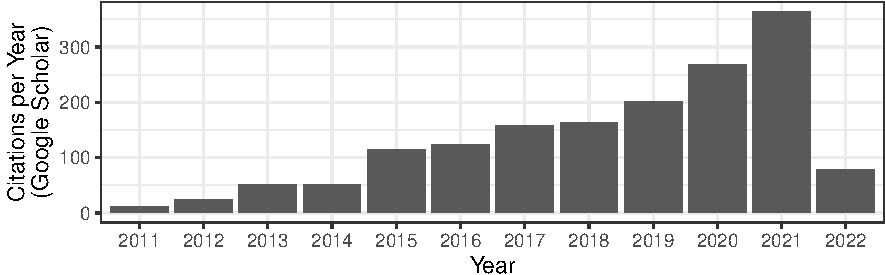
\includegraphics{publication_files/figure-latex/unnamed-chunk-2-1} \end{center}

\hypertarget{working-papers-under-revision-or-review}{%
\subsection{\texorpdfstring{\textbf{Working Papers under Revision or
Review}}{Working Papers under Revision or Review}}\label{working-papers-under-revision-or-review}}

\begingroup
\setlength{\parindent}{-0.5in}
\setlength{\leftskip}{0.5in}

\hypertarget{refs_journalspress}{}

\vspace{7mm}

\hypertarget{refereed-journal-papers---2023}{%
\subsection{\texorpdfstring{\textbf{Refereed Journal Papers -
2023}}{Refereed Journal Papers - 2023}}\label{refereed-journal-papers---2023}}

\hypertarget{refs_journals2023}{}

\hypertarget{refereed-journal-papers---2022}{%
\subsection{\texorpdfstring{\textbf{Refereed Journal Papers -
2022}}{Refereed Journal Papers - 2022}}\label{refereed-journal-papers---2022}}

\hypertarget{refs_journals2022}{}

\hypertarget{refereed-journal-papers---2021}{%
\subsection{\texorpdfstring{\textbf{Refereed Journal Papers -
2021}}{Refereed Journal Papers - 2021}}\label{refereed-journal-papers---2021}}

\hypertarget{refs_journals2021}{}

\vspace{7mm}

\hypertarget{refereed-journal-papers---2020}{%
\subsection{\texorpdfstring{\textbf{Refereed Journal Papers -
2020}}{Refereed Journal Papers - 2020}}\label{refereed-journal-papers---2020}}

\hypertarget{refs_journals2020}{}

\vspace{7mm}

\hypertarget{refereed-journal-papers---2019}{%
\subsection{\texorpdfstring{\textbf{Refereed Journal Papers -
2019}}{Refereed Journal Papers - 2019}}\label{refereed-journal-papers---2019}}

\hypertarget{refs_journals2019}{}

\vspace{7mm}

\hypertarget{refereed-journal-papers---2018}{%
\subsection{\texorpdfstring{\textbf{Refereed Journal Papers -
2018}}{Refereed Journal Papers - 2018}}\label{refereed-journal-papers---2018}}

\hypertarget{refs_journals2018}{}

\vspace{7mm}

\hypertarget{refereed-journal-papers---2017-and-prior}{%
\subsection{\texorpdfstring{\textbf{Refereed Journal Papers - 2017 and
Prior}}{Refereed Journal Papers - 2017 and Prior}}\label{refereed-journal-papers---2017-and-prior}}

\hypertarget{refs_journals2017}{}

\clearpage

\hypertarget{papers-in-refereed-conference-proceedings}{%
\subsection{\texorpdfstring{\textbf{Papers in Refereed Conference
Proceedings}}{Papers in Refereed Conference Proceedings}}\label{papers-in-refereed-conference-proceedings}}

\hypertarget{refs_proceedings}{}

\vspace{7mm}

\hypertarget{conference-presentations-coauthored}{%
\subsection{\texorpdfstring{\textbf{Conference Presentations
Coauthored}}{Conference Presentations Coauthored}}\label{conference-presentations-coauthored}}

\hypertarget{refs_confco}{}

\vspace{7mm}

\hypertarget{work-not-peer-reviewed}{%
\subsection{\texorpdfstring{\textbf{Work Not Peer
Reviewed}}{Work Not Peer Reviewed}}\label{work-not-peer-reviewed}}

\hypertarget{refs_notpeer}{}

\clearpage

\vspace{7mm}

\hypertarget{disertation}{%
\subsection{\texorpdfstring{\textbf{Disertation}}{Disertation}}\label{disertation}}

\hypertarget{refs_student}{}

\vspace{7mm}

\hypertarget{online-ebook}{%
\subsection{\texorpdfstring{\textbf{Online
eBook}}{Online eBook}}\label{online-ebook}}

\hypertarget{refs_ebook}{}

\endgroup


\end{document}

%\clearpage\end{CJK*}                              % if you are typesetting your resume in Chinese using CJK; the \clearpage is required for fancyhdr to work correctly with CJK, though it kills the page numbering by making \lastpage undefined
\end{document}


%% end of file `template.tex'.
